\chapter{量子光通信的理论基础}




\section{电磁场的量子态描述}



\section{经典光通信的接收方案}

\subsection{引言}
在经典光通信中,有三类常见的接收方案,他们分别是
直接检测、零差接收和外差接收。
这三种接收方案受散粒噪声的制约,
使得每一种接收方案存在一个经典极限
——标准量子极限(Standard Quantum Limit)。
接下来,我们简单介绍一下每一种接收方案的具体实现和它们的性能。

\subsection{直接检测}

在所有的调制方案中,有一类采用脉冲的有无对信息进行编码,
比如开关键控(OOK)和脉冲位置调制(PPM)。
OOK调制将符号0编码为没有光脉冲,
而将符号1编码为有脉冲;PPM调制则将信息编码到脉冲所在的位置上。
对于这样一类的调制方案,经典光通信中常采用直接检测方案进行探测。
如图\ref{fig:DD}所示,直接检测方案直接探测信号光的强度,
来判断是否存在光脉冲或者光脉冲的幅度。
这种方案可以利用一个光电探测器或单光子探测器实现。
探测器可以输出探测到的光子数目,理想情况下,
对于给定的相干态,探测到$n$个光子的概率
\begin{equation}
\Pr(N = n| \ket{\alpha}) = \frac{|\alpha|^{2n}}{n!} e^{-|\alpha|^2}
\label{eq:dd-prob}
\end{equation}
一般地,对于信号矢态为$\ket{\phi}$的情况下,检测概率为
\begin{equation}
\Pr(N = n| \ket{\phi}) = |\bra{n}\ket{\phi}|^2
\end{equation}



\begin{figure}
\centering
  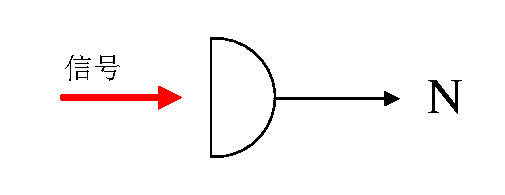
\includegraphics[scale=1]{figures/chap2/DD.pdf}
  \caption{直接检测示意图}
  \label{fig:DD}
\end{figure}


\subsection{零差接收}
零差接收机是一种相干检测方案,如图\ref{fig:HD}所示,
是一种平衡零差接收方案。这种接收方案和直接检测不同的是,
需要一个本振。对于零差接收本振频率和信号频率一致。
通常本振强度$a_{LO}$远大于信号强度$a_s$,
两路信号通过一个50:50的分束器,
在两个输出口得到两路新的信号$a_+$和$a_-$,满足关系式
\begin{equation}
a_\pm = \frac{a_s \pm a_{LO}}{\sqrt{2}}.
\end{equation}
这两路信号被光电探测器接收,得到两路光电流$i_\pm$。
这两路电流通过一个放大系数为$K$的差分放大器,最后通过一个
低通滤波器积分得到输出统计量
\begin{equation}
a_\theta = \frac{N_+ - N_-}{2\sqrt{N_{LO}}}.
\end{equation}
这里假定所有的器件都是理想的。当$N_{LO} \rightarrow \infty$时,
输出统计量服从高斯分布
\begin{equation}
a_\theta \sim N(Re(ae^{-j\theta}), \frac{1}{4}).
\end{equation}
用量子力学算符可以描述为
\begin{equation}
\hat{a}_\theta = Re(\hat{a}e^{-j\theta}).
\end{equation}


\begin{figure}
\centering
  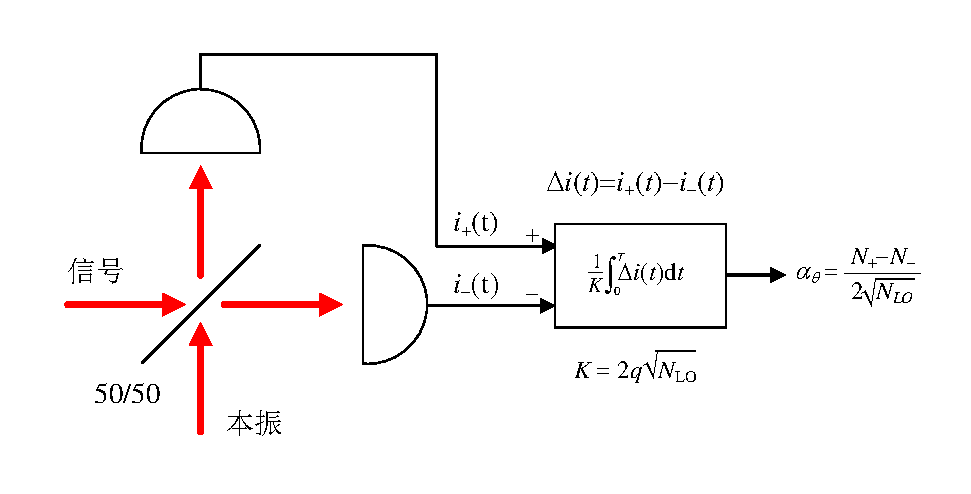
\includegraphics[scale=1]{figures/chap2/homodyne-receiver.pdf}
  \caption{平衡零差检测示意图}
  \label{fig:HD}
\end{figure}

\subsection{外差接收}




\section{量子检测与估计理论}

\subsection{最优检测}






\subsection{平方根检测}







\section{现有的量子接收机简介}

\subsection{二进制信号量子接收机}




\subsection{PSK信号量子接收机}





\subsection{其它类型量子接收机}






\section{量子信道编码理论}

\subsection{Holevo容量}






\subsection{常见的量子编码方案}





